\chapter{Interfejs użytkownika}
\section{Widok strony głównej}
Widok strony głównej zależy od tego czy sesja użytkownika jest autoryzowana. Przed zalogowaniem wyświetlane są informacje na temat aplikacji. Po zalogowaniu zobaczyć możemy przyciski przekierowujące użytkownika do głównych podmiotów aplikacji.
\begin{figure}[h!]
	\centering
	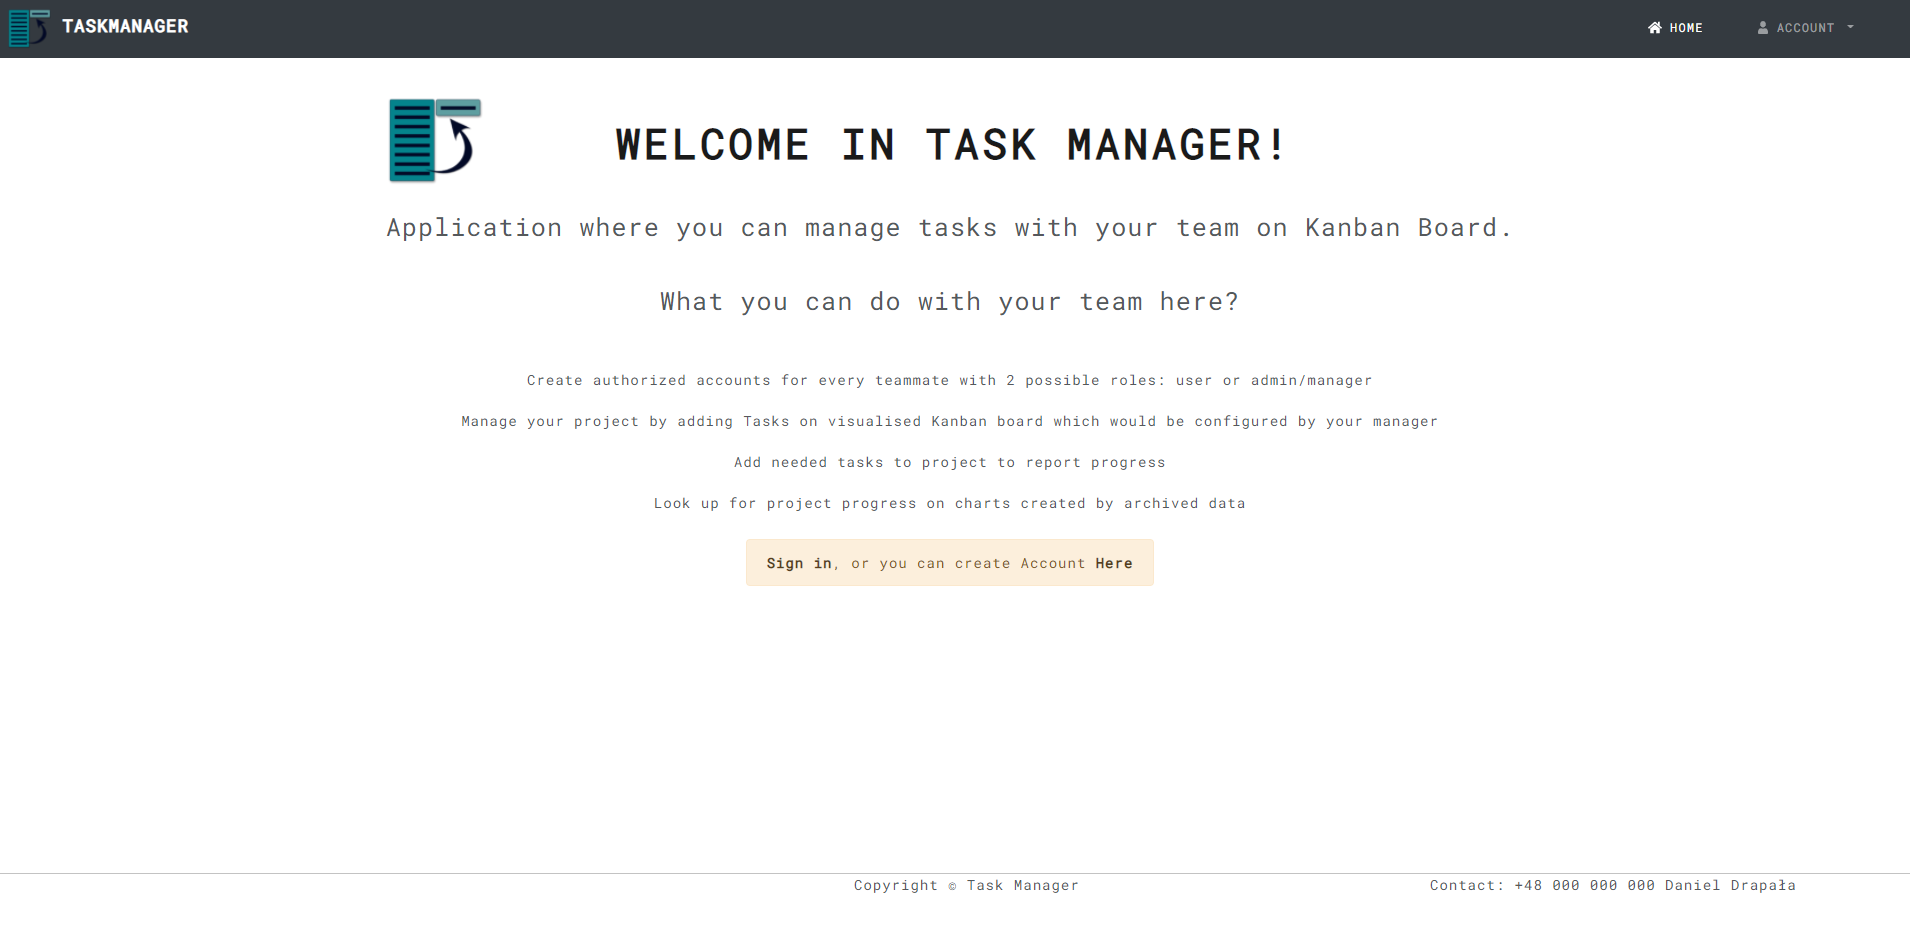
\includegraphics[width=0.90\textwidth]{home-not-auth}
	
	\caption{Widok strony głównej przed zalogowaniem.}
	\label{not-auth-home}
\end{figure}

\begin{figure}[h!]
	\centering
	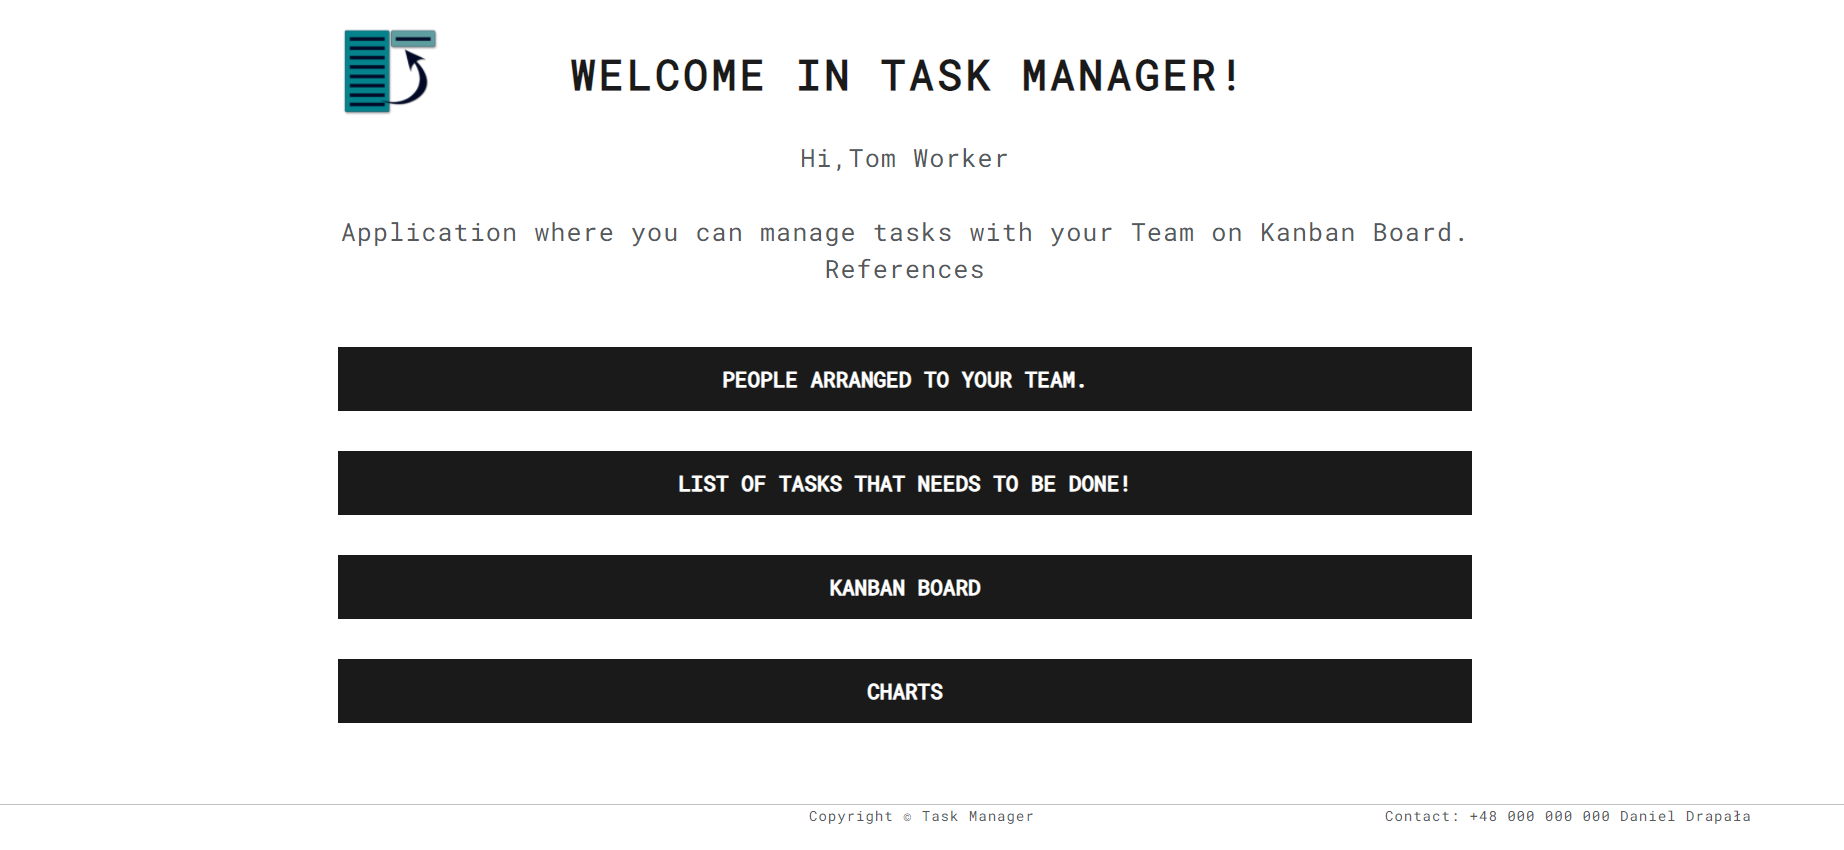
\includegraphics[width=0.90\textwidth]{home-auth}
	
	\caption{Widok strony głównej po zalogowaniu.}
	\label{auth-home}
\end{figure}

\section{Widok nagłówka strony}
Na rysunku \ref{navbar-states} przedstawiony został widok nagłówka, który jest elementem umiejscowionym na górze strony na każdym dostępnym widoku. Posiada przyciski przekierowujące do innych podmiotów aplikacji.
Stan z najmniejszą liczbą dostępnych opcji jest wyświetlany dla użytkownika niezalogowanego. Jedynymi możliwościami jest wtedy strona startowa, strona rejestracyjna oraz strona z formularzem logowania.
Drugi stan jest wyświetlany dla administratora, który oprócz funkcji użytkownika posiada również zakładkę \linebreak \textit{Administration}, gdzie może przejść do zarządzania użytkownikami lub tablicą.
Trzeci stan dla użytkownika o zwykłych uprawnieniach składa się z odnośnika do strony startowej, ale również wszystkie dostępne podmioty strony: 
\begin{itemize}
	\item lista użytkowników, która jest jedynie listą podglądową, nie posiada ona licznych funkcji jak lista dla administratora \ref{users-list}
	\item tablica kanban
	\item lista zadań
	\item wykresy
	\item ustawienia konta
	\item zmiana hasła
	\item aktywne, zapisane sesje
	\item przycisk wylogowania się z sesji
\end{itemize}
\begin{figure}[h!]
	\centering
	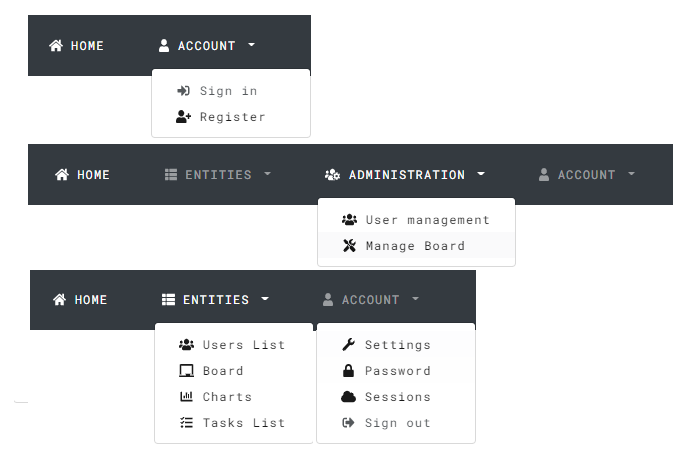
\includegraphics[width=0.90\textwidth]{navbar-states}
	
	\caption{Widok nagłówka w trzech stanach.}
	\label{navbar-states}
\end{figure}
\clearpage

\section{Widoki rejestracji i logowania}
Widok rejestracji i logowania składają się z formularza do wypełnienia, aby dostarczyć serwerowi odpowiednie dane do autoryzacji.
\begin{figure}[h!]
	\centering
	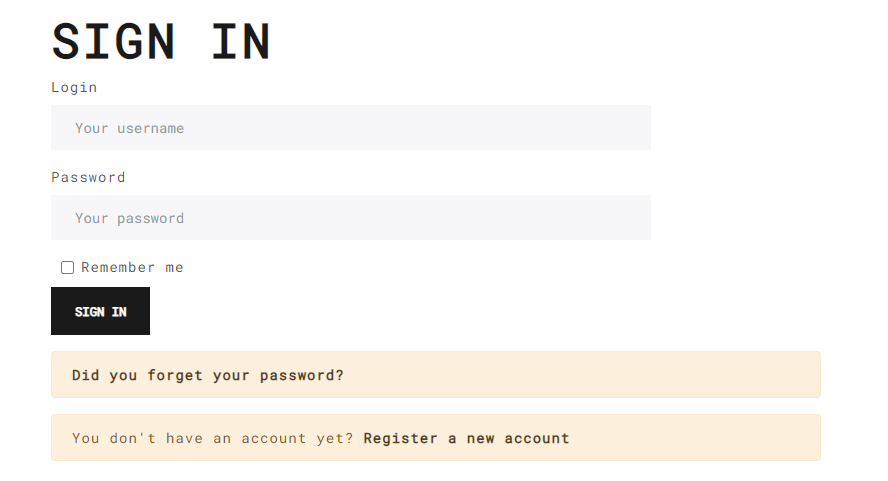
\includegraphics[width=0.60\textwidth]{loginstate}
	
	\caption{Widok logowania.}
	\label{login-state}
\end{figure}

\begin{figure}[h!]
	\centering
	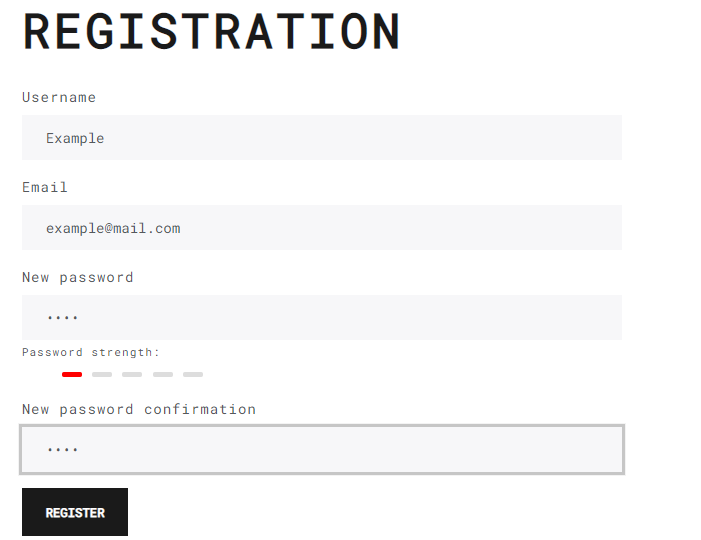
\includegraphics[width=0.60\textwidth]{register}
	
	\caption{Widok rejestracji nowego użytkownika.}
	\label{register-state}
\end{figure}
\clearpage
\subsection{Widok zmiany hasła}
Widok \ref{change-pass} prezentuje formularz ze zmianą hasła. Ciekawym dodatkiem wprowadzonym do danego widoku jest pasek siły hasła. Jest to styl składający się z pięciu bloków kolorowanych odpowiednio na kolor czerwony pomarańczowy i zielony w zależności od tego jak silne hasło zostało wprowadzone. Odpowiedzialna za kolorowanie tych bloków metoda analizuje wprowadzone hasło pod kątem skomplikowania za pomocą wyrażeń regularnych.
Sprawdzane zostaje czy w haśle użyty został co najmniej jeden symbol specjalny, jedna wielka litera, jedna mała litera oraz liczba.
\begin{figure}[h!]
	\centering
	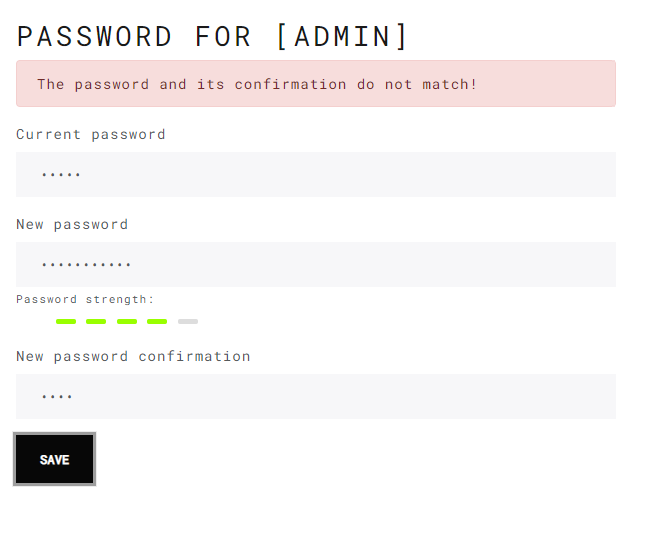
\includegraphics[width=0.90\textwidth]{change-pass}
	
	\caption{Widok zmiany hasła.}
	\label{change-pass}
\end{figure}
\clearpage

\section{Widok listy zadań i użytkowników}
Widok list dostępnych z aplikacji składają się z responsywnych list, które wyświetlają informacje wyciągane z bazy danych w postaci stron. Serwis wysyłający zapytanie o listę użytkowników bądź zadań dołącza informacje o ograniczeniach. Podane listy ograniczone są do dwudziestu pięciu elementów na stronę. Serwer wysyła maksymalną liczbę elementów oraz informację na temat liczby pozostałych elementów. Za pomocą tych danych otrzymujemy listę podzieloną na strony. Przejście na kolejną stronę skutkowałoby wysłaniem zapytania o kolejne dwadzieścia pięć elementów.
\begin{figure}[h!]
	\centering
	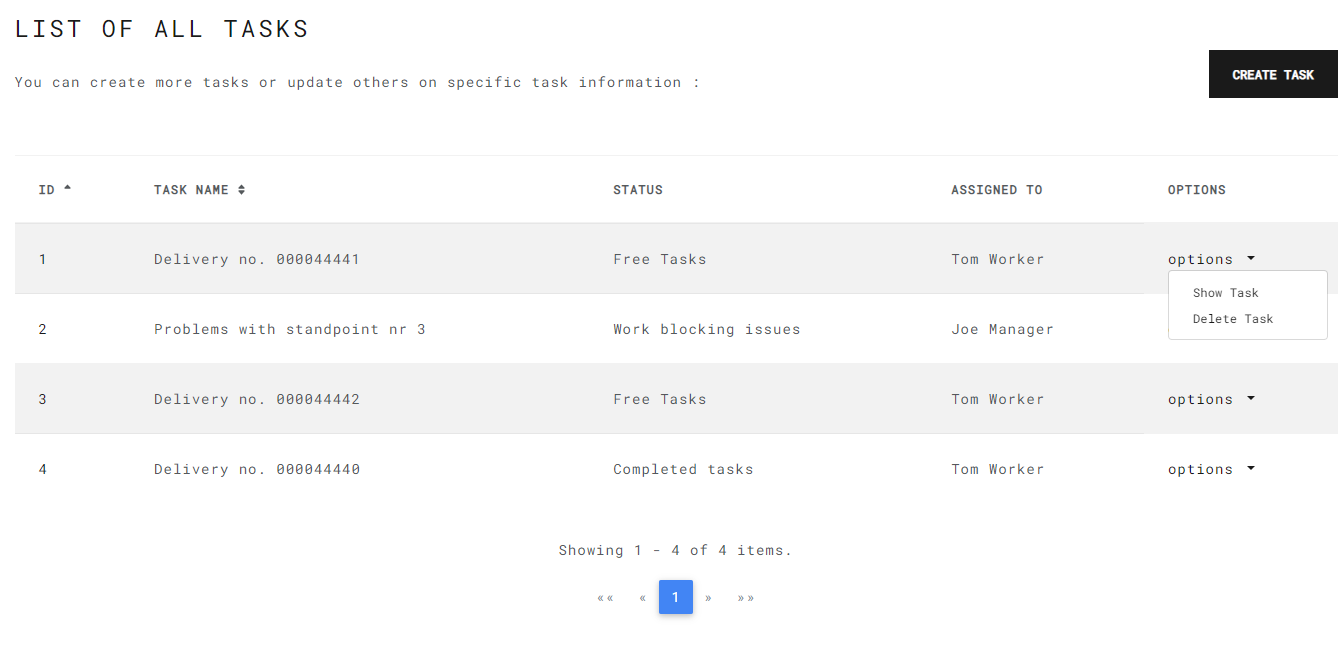
\includegraphics[width=0.90\textwidth]{taskslist}
	
	\caption{Widok listy zadań.}
	\label{tasklist}
\end{figure}

\begin{figure}[h!]
	\centering
	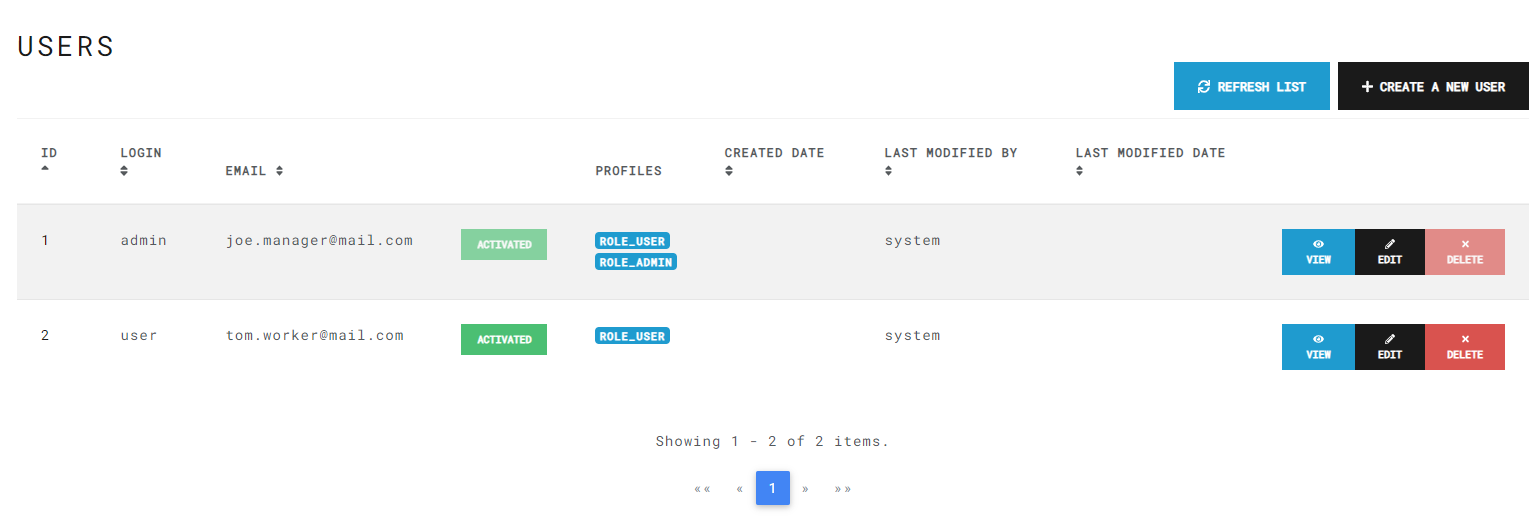
\includegraphics[width=0.90\textwidth]{users-lists}
	
	\caption{Widok listy użytkowników dla administratora.}
	\label{users-list}
\end{figure}
\clearpage

\section{Widok Statystyk}
Statystyki przedstawione są na przejrzystym panelu. Na początku strony wyświetlane zostają informacje na temat projektu wraz z wykresami kołowymi przedstawiające ogólny postęp wykonanych zadań.
Niżej widnieje lista użytkowników oraz lista zadań. Po wybraniu odpowiednich rekordów z listy wyświetlane zostają po kolei wykresy dla poszczególnych zadań jak na rysunku \ref{scrolledstatistics}.
\begin{figure}[h!]
	\centering
	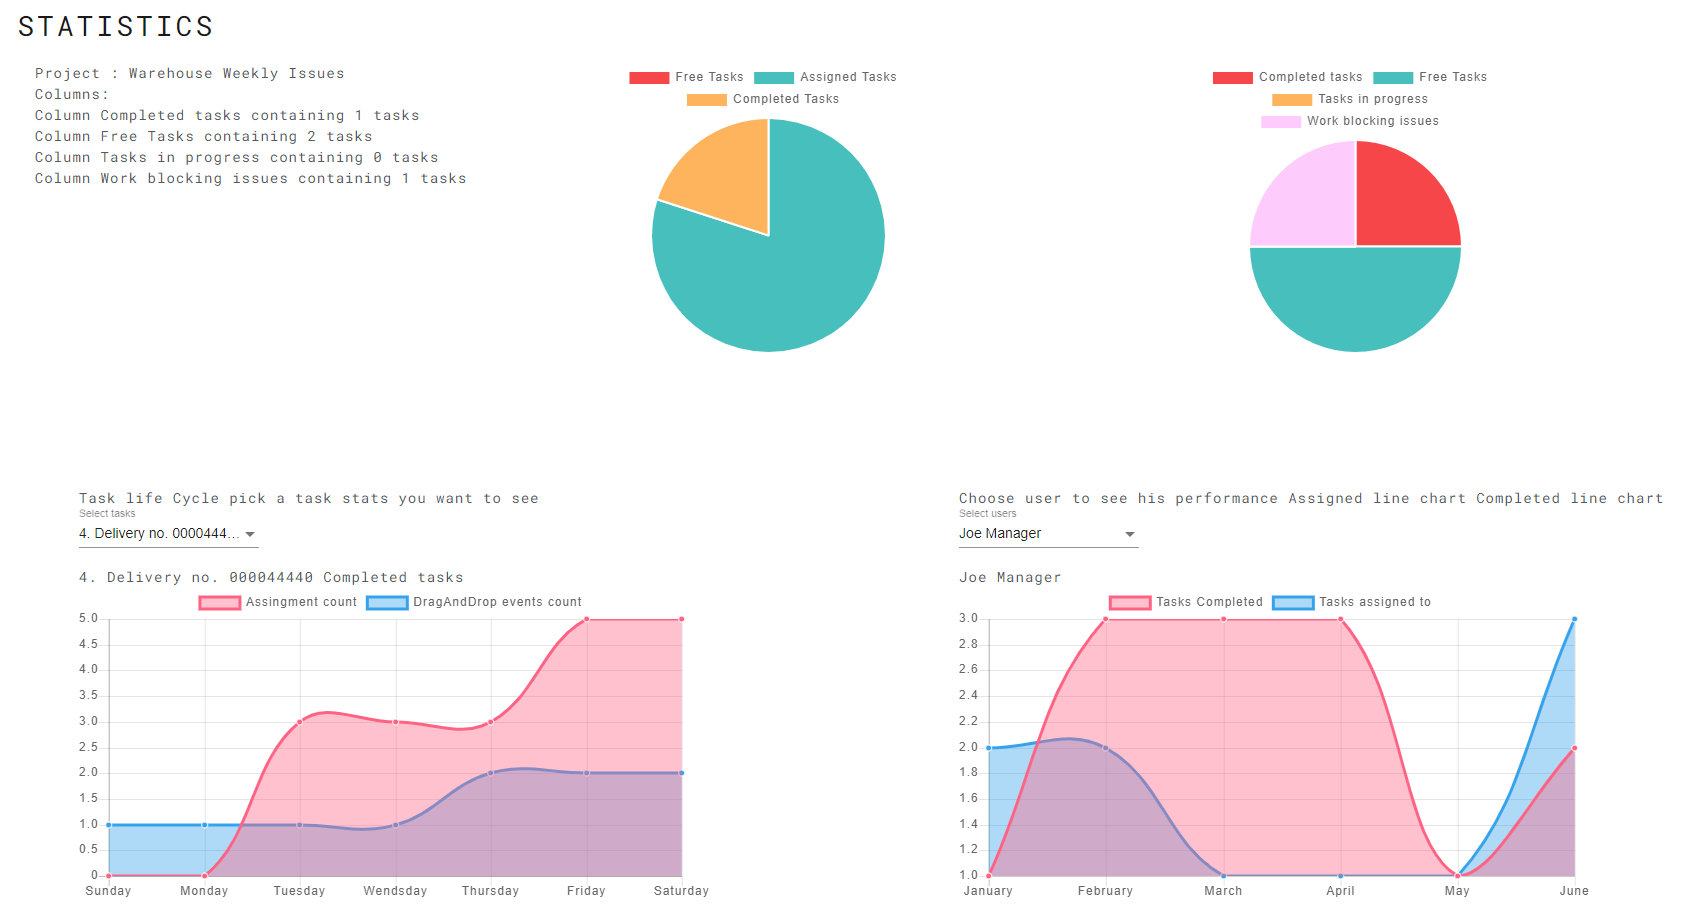
\includegraphics[width=0.90\textwidth]{statistics}
	
	\caption{Widok statystyk.}
	
	\label{statistics}
\end{figure}

\begin{figure}[h!]
	\centering
	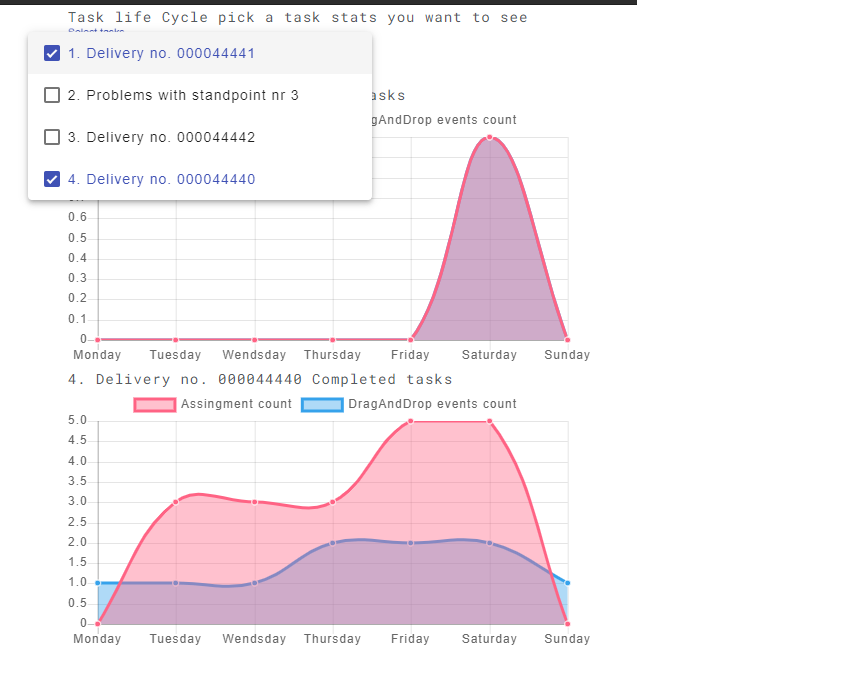
\includegraphics[width=0.60\textwidth]{scrolledstatistics}
	
	\caption{Widok statystyk dla wymienionych z listy zadań.}
	
	\label{scrolledstatistics}
\end{figure}
\clearpage
\section{Widoki związane z tablicą}
\begin{figure}[h!]
	\centering
	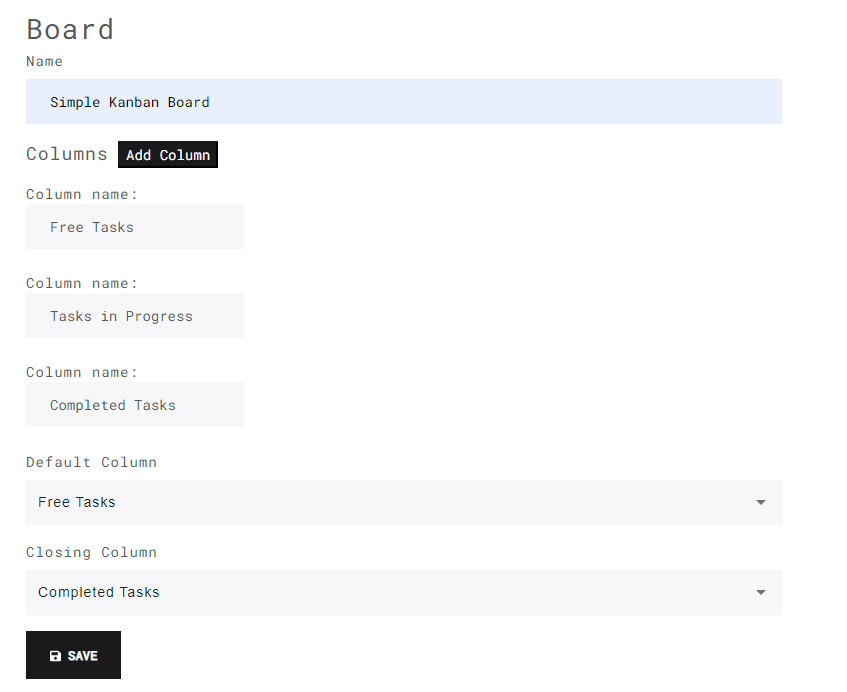
\includegraphics[width=0.60\textwidth]{addboard}
	
	\caption{Widok dodawania tablicy.}
	\label{addb}
\end{figure}


\begin{figure}[h!]
	\centering
	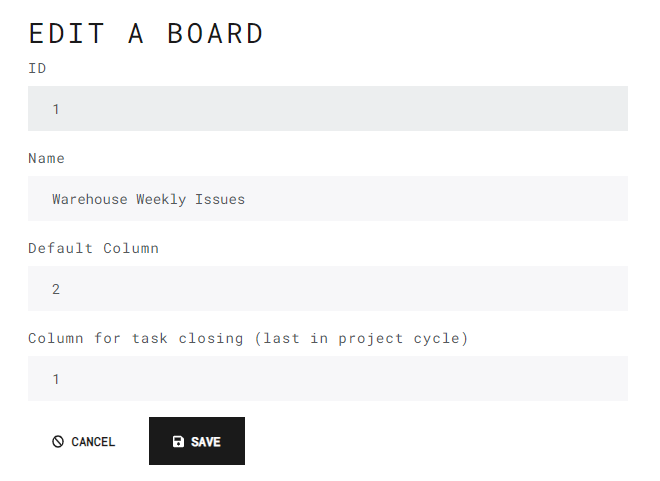
\includegraphics[width=0.60\textwidth]{boardedit}
	
	\caption{Widok edycji tablicy.}
	\label{boardedit}
\end{figure}
\clearpage
\paragraph{Główny widok tablicy}
Widok tablicy składa się z kontenera o kolorze \textit{cadetblue}. Przechowuje on trzy kontenery odpowiadające kolumną tablicy \textit{kanban}.
Zadania wyświetlane są w postaci białych bloków, które przedstawiają najważniejsze informacje:
\begin{itemize}
	\item nazwę zadania
	\item do kogo zadanie zostało przypisane (zaznaczone na czerwono jeśli przypisane zostało do użytkownika przeglądającego tablicę)
	\item przeniesienie zadania do kolumny kończącej zadanie edytuje styl bloku na zielony i dopisana zostaje informacja, że podane zadanie zostało wykonane
\end{itemize}
\begin{figure}[h!]
	\centering
	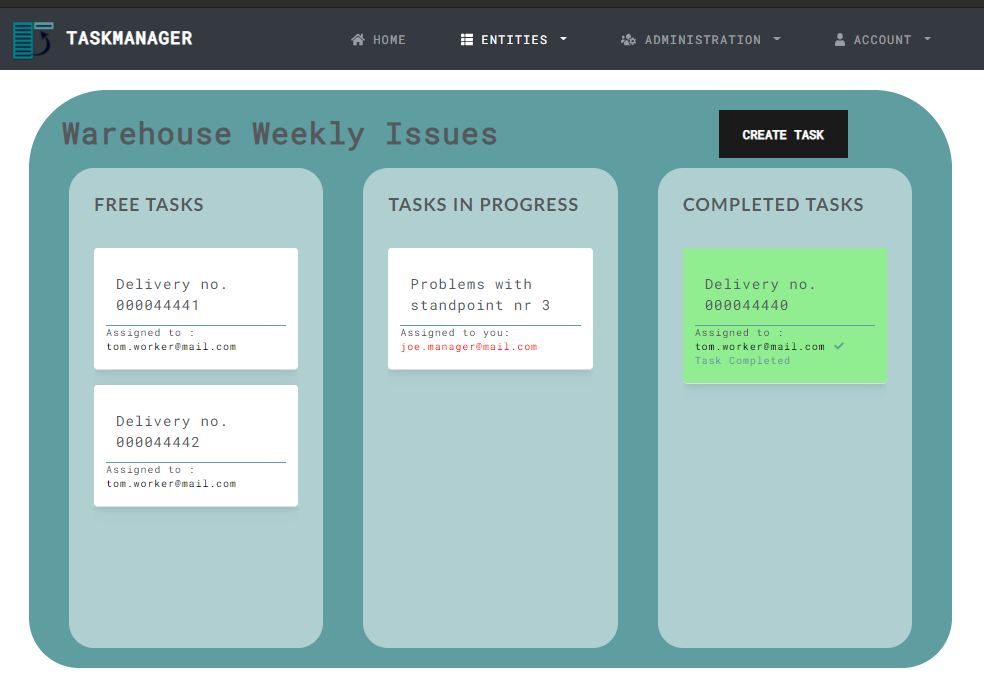
\includegraphics[width=0.90\textwidth]{kanban-view}
	
	\caption{Widok tablicy.}
	\label{board}
\end{figure}
\clearpage
\section{Widok Szczegółów Zadania}
Widok \ref{taskcomm} przedstawiający szczegóły zadania za pomocą formularza, który może zostać w każdej chwili zaktualizowany. W szczegółach zadania możemy wprowadzać odpowiednio komentarze dotyczące zadania. 
\begin{figure}[h!]
	\centering
	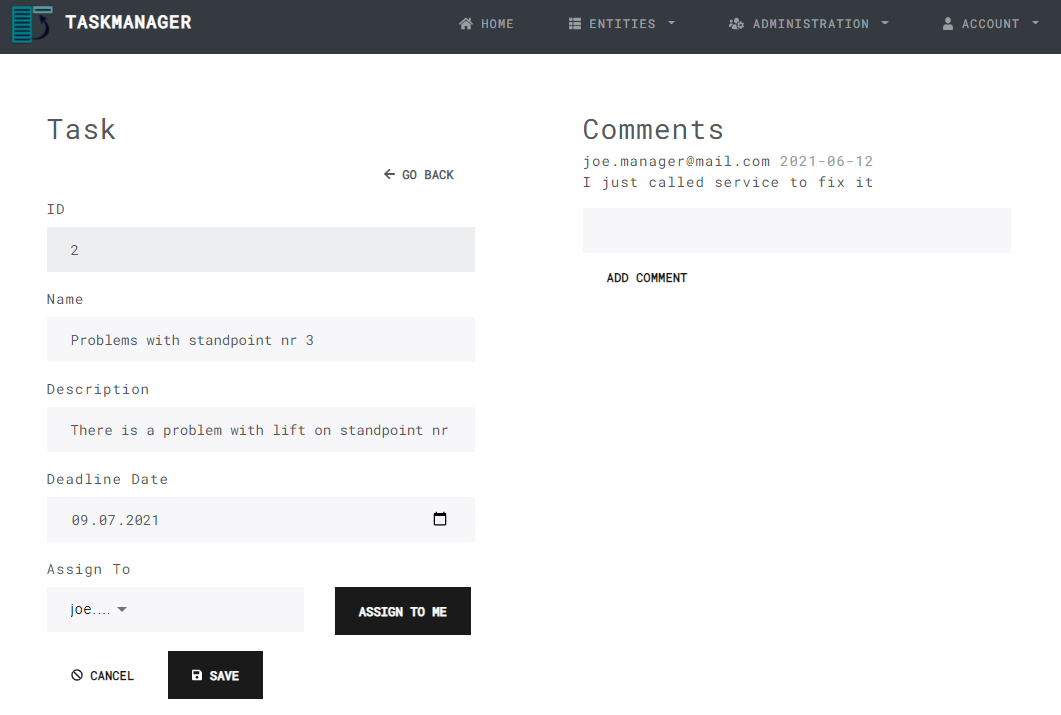
\includegraphics[width=0.90\textwidth]{taskcomm}
	
	\caption{Widok szczegółów zadania.}
	\label{taskcomm}
\end{figure}
